\documentclass[a4paper,12pt]{article}
\usepackage[russian]{babel}
\usepackage[utf8]{inputenc}
\usepackage{amsmath}
\usepackage{graphicx}
\usepackage[perpage]{footmisc} 
\usepackage{braket}
\usepackage{fullpage}

\renewcommand{\baselinestretch}{1.5}
\newcommand{\vect}[1]{\boldsymbol{#1}}


\title{Высокоэнергетическое рассеяние без разложения по парциальным волнам.}
\author{.}

\begin{document}
	
	
	%\pagestyle{plain}
  \begin{titlepage}
  
  \begin{center}
	Министерство образования и науки \\
	Российской Федерации \\ 
	Федеральное агенство по образованию \\ 
	Федеральное государственно бюджетное образовательное \\
	учреждение высшего профессионального образования \\
	% \end{center}
	%   \begin{center}
	Национальный исследовательский ядерный университет \\
	«МИФИ» \\
	% \end{center}
	% \begin{center}
	Факультет экспериментально и теоретической физики
	Кафедра теоретической ядерной физики №32
	\end{center}
	
	\vspace{1cm}
	
	\begin{center}\Large
	Диплом на соискание степени бакалавра по теме: \\
	\bf{Решение квантовой задачи рассеяния на основе дискретизации континуума без использования парциально-волновых разложений.}
  \end{center}
  
  \vspace{1cm}
	
	\begin{flushright}
	\textbf{Выполнил}: \\
	студент группы Т8-32 \\
	Кельвич Станислав Александрович \\
	\vspace{1cm}
	\textbf{Научный руководитель}: \\
	д.ф.-м.н. старший научный сотрудник \\
	НИИ Ядерной Физики МГУ \\
	Кукулин Владимир Иосифович \\
	\end{flushright}
	
	\vspace{1.5cm}
	\begin{center}
	  Москва, 2010
	\end{center}
	
  \end{titlepage}
	\pagebreak
	
	\setcounter{page}{2}
	\tableofcontents
    \pagebreak
     
	\begin{abstract}
		В данной работе получена конечномерная аппроксимация операторов рассеяния и уравнения Липпмана-Швингера путем перехода из базиса плоских волн в квазидискретный базис волновых пакетов. В таком представлении функция Грина свободной частицы интегрируется аналитически, что существенно упрощает численное решение уравнений теории рассеяния. Впервые использованы многомерные стационарные волновые пакеты, что позволяет избежать разложения волновых функций по парциальным волнам и тем самым упростить точное решение задачи рассеяния при промежуточных энергиях.
	\end{abstract}
	\pagebreak

	\section{Введение}
При небольших энергиях порядка десятка МэВ вклад в процесс рассеяния даёт лишь небольшое количество парциальных амплитуд. В соответствии с этим метод разложения по парциальным волнам является эффективным для расчетов при таких энергиях. С другой стороны при промежуточных и высоких энергиях порядка сотен МэВ вклад в амплитуду рассеяния дает большое количество парциальных волн. Такие вклады являются сильно осциллирующими функциями угла рассеяния при этом результирующая амплитуда является более гладкой функцией. И поэтому для того, чтобы избегать больших пограешностей в расчете наблюдаемых (сечений и т.д.) приходится не только учитывать много парциальных волн, но и каждый фазовый сдвиг считать с весьма высокой точностью, что сильно усложняет всю численную схему. Для устранения этих трудностей ряд авторов предложили отказаться от использования разложения по парциальным волнам в случае промежуточных энергий, интегрируя непосредственно уравнение Липпманна-Швингера в импульсном представлении\cite{elster}.

Необходимость пользоваться состояниями непрерывного спектра также вызывает трудности из-за сложных граничных условий, которым должны удовлетворять волновые функции, особенно в задачах нескольких частиц, где имеется несколько континуумов, часто налагающихся друг на друга. Для решения этих проблем был предложен общий подход\cite{kuku2}\cite{kuku1}, основанный на пакетной  дискретизации операторов теории рассеяния. Суть этого метода заключается в том, что весь континуум энергий разбивается на полосы малой ширины и в пределах таких интервалов строятся стационарные волновые пакеты из функций свободного движения. Затем операторы рассеяния проектируются в это конечномерное представление.

В данной работе метод, который авторы \cite{kuku2}\cite{kuku1} применяли для дискретизации одномерного континуума обобщается для решения трехмерной задачи рассеяния, обходя разложение по парциальным волнам. %При этом получается трёхмерная сетка дискретных значений импульса. 
Таким образом используя это представление можно отказаться и от разложения по парциальным волнам и от состояний непрерывного спектра. В настоящей работе получены формулы для перехода в такое представление, явное выражение для функции Грина свободной частицы и написан дискретный аналог трехмерного уравнения Липпманна-Швингера. В качестве численных иллюстраций расчитано сечение N-N рассеяния на гауссовом потенциале и потенциале Мальфлие-Тьона. Произведено сравнение результатов расчета на основе данного метода с методом фазовых функций\cite{babik}.

% Для решения возникающих при этом уравнений необходимы большие вычислительные мощности, и проведение таких расчетов на персональных компьютерах возможно лишь в небольшом числе случаев. В связи со все возрастающей доступностью параллельных вычислений (grid-сети, кластеры, суперкомпьютеры) возникает проблема разработки методов и алгоритмов решения задач рассеяния в многопоточном режиме. При этом возможно существенно увеличить число задач, поддающихся вычислению ab initio.

\newline
	\section{Базис стационарных волновых пакетов.}
Рассмотрим процесс рассеяния двух частиц. Гамильтониан этой системы запишем выделив взаимодействие и гамильтониан свободной частицы:
\[
	H = H_0 + V,
\]
где потенциал $V$ – короткодействующий с характерным размером $a$. Собственные функции $H_0$ это состояния рассеяния (то есть состояния непрерывного спектра) с определенным импульсом, выберем их нормированными на дельта-функцию:
\[
	\braket{\vect{r}|\vect{q}} = \frac{1}{(2\pi)^{3/2}}e^{i\vect{q}\vect{r}} 
\]\[
	\braket{\vect{q}|\vect{q'}} = \delta(\vect{q} - \vect{q'})
\]

%	\subsection{Волновые пакеты.}
Перейдем теперь от точных волновых функций свободного движения к стационарным волновым пакетам. Введем разбиение $D$ трехмерного импульсного пространства на малые области и перенумеруем эти области индексом $\alpha$. Волновым пакетом мы будем называть сумму всех $\ket{\vect{q}}$, импульс которых попадает в заданную область $D_\alpha$. При этом интегрирование произведем с весовой функцией $f(q)$:
\[
	\ket{\alpha} = \frac{1}{\sqrt{\mu_\alpha}} \int\limits_{D_\alpha} f(q) \ket{\vect{q}} d^3q
\]
Коэффициент $\mu_\alpha$ найдем из условия нормировки:
\[
	\braket{\alpha|\beta} = \frac{1}{\sqrt{\mu_\alpha \mu_\beta}}  \int\limits_{D_\alpha}  \int\limits_{D_\beta} f(q)f^\dagger(q') \delta(\vect{q} - \vect{q'}) d^3q d^3q' = 1
\]
Отсюда имеем:
\[
	\mu_\alpha =  \int\limits_{D_\alpha} |f(q)|^2 d^3q
\]
Таким образом мы заменили непрерывный спектр состояний свободного движения на квазидискретный и полученный набор собственных функций является ортонормированным, как и в обычном гильбертовом пространстве. Полным этот набор функций становится в пределе $D_\alpha \to 0$:
\[
	\braket{\alpha|\beta} = \delta_{\alpha,\beta}
\]\[
	\sum\limits_\alpha \ket{\alpha}\bra{\alpha} = P
\]

Сетку разбиения удобно выбирать так, чтобы её поверхности уровня совпадали с поверхностями уровня системы координат в которых производится интегрирование. Например, в случае декартовых координат $d^3q = dq_xdq_ydq_z$ логично выбрать прямоугольную решетку. В данном случае более удобным будет интегрирование в сферической системе координат поскольку энергия зависит только от одной координаты – модуля импульса, кроме того явно выделен азимутальный угол и это существенно упрощает решение задачи рассеяния со сферически-симметричным потенциалом. Таким образом в качестве $D_\alpha$ выбирается следующая область:
\[
 D_{\alpha(i,j,k)} = \big\{ \: (k,\theta,\varphi) \: \big| \: q \in [q_i,q_{i+1}], \theta \in [\theta_j,\theta_{j+1}], \varphi \in [\varphi_k,\varphi_{k+1}] \: \big\} 
\]\[
 \text{ где } \alpha \text{ нумерует сочетания } \big\{ (0,0,0), \; ... \; , (i_{max},j_{max},k_{max}) \big\}
\]
\newline
	\subsection{Волновые пакеты в случае аксиальной симметрии.}
В случае сферически-симметричного потенциала результат решения задачи не должен зависеть от азимутального угла. При этом удобно использовать смешанное представление, в котором угол $\varphi$ – непрерывная переменная, а модуль $|\vect{q}|$ и полярный угол – дискретные. Интегрирование проведем в сферических координатах. Итого, имеем следующее представление:

\[
	\ket{\alpha,\varphi} = \frac{1}{\sqrt{\mu_\alpha}} \int\limits_{D_\alpha} f(q) \ket{\vect{q}} q^2 \,dq \,d(-\cos\theta)
\]
\[
	\mu_\alpha =  \int\limits_{D_\alpha} |f(q)|^2 q^2 \,dq \,d(-\cos\theta)
\]
Определенные так волновые пакеты нормированны следующим условием:
\[
	\braket{\alpha,\varphi|\beta,\varphi'} = \delta_{\alpha,\beta}\delta(\varphi'-\varphi)
\]\[
	\sum\limits_\alpha \int\limits_0^{2\pi} \,d \varphi \ket{\alpha,\varphi}\bra{\alpha,\varphi} = 1
\]
Теперь рассмотрим подробнее выбор узлов решетки:
\[
 \text{ узлы решетки по }q: \;\; q_i, \;\;\; i=\overline{0,M}
\]\[
 \text{ узлы решетки по }\theta: \;\;  \theta_j, \;\;\; j=\overline{0,N}
\]
На каждом интервале выберем средний элемент
\[
 q_i^* \in [q_i,q_{i+1}], \;\;\; i=\overline{0,M-1}
\]\[
 \theta_j^* \in [\theta_j,\theta_{j-1}], \;\;\; j=\overline{0,N-1}
\]
и перейдем от двойного индекса $(i,j)$ к одинарному
\[
	\alpha = \overline{0,N M-1},
\]\[
	i = [\alpha/N], \;\;\; j = \alpha \bmod N,
\]\[
	\vect{q^*_\alpha} = (q_i^*,\theta_j^*),
\]
где $x \bmod y$ – остаток от деления $x$ на $y$, а $[x/y]$ – целая часть деления. Если рассматривать величины $(q_i^*,\theta_j^*)$ как элементы матрицы, то такое преобразование эквивалетно следующему изменению индексов в матрице:
\[
\begin{pmatrix} 
a_{00}    & a_{01}    & \dots  & a_{0,N-1}  \\ 
a_{10}    & a_{11}    & \dots  & a_{1,N-1}  \\ 
\vdots    & \vdots    & \ddots & \vdots     \\ 
a_{M-1,0} & a_{M-1,1} & \dots  & a_{M-1,N-1}  
\end{pmatrix}  \longrightarrow  \begin{pmatrix} 
a_{0}      & a_{1}        & \dots   & a_{N-1}  \\  
a_{N}      & a_{N+1}      & \dots   & a_{2N-1} \\ 
\vdots     & \vdots       & \ddots  & \vdots   \\
a_{(M-1)N} & a_{(M-1)N+1} & \dots   & a_{NM-1} 
\end{pmatrix}
\]
\newline
\subsection{Операторы в представлении волновых пакетов.}

Теперь получим выражение операторов в представлении волновых пакетов (ВП) через операторы в импульсном представлении. Пусть дан оператор с матричными элементами в импульсном представлении
\[
	A(\vect{q'},\vect{q}) \equiv \bra{\vect{q'}}A\ket{\vect{q}}
\] и оператор с матричными элементами в представлении ВП \[
  A_{\alpha\beta}(\varphi',\varphi) \equiv \bra{\alpha,\varphi'}A\ket{\beta,\varphi}.
\]
Переход от одного представления к другому осуществляется по стандартной формуле:
\[
	A_{\alpha\beta}(\varphi',\varphi) = \int d^3q \int d^3q' \braket{\alpha,\varphi'|\vect{q'}} A(\vect{q'},\vect{q}) \braket{\vect{q}|\beta,\varphi}.
\] 
Перекрывание ВП и плоской волны вычисляется исходя из определения ВП:
\[
 \braket{\vect{q}|\alpha,\varphi'} = \frac{f(q)}{\sqrt{\mu_\alpha}} \delta_{\alpha,\{\vect{q}\}} \delta(\varphi'-\varphi)
\]
Здесь и далее под $\{\vect{q}\}$ подразумевается номер интервала, в который попадает этот вектор. Подставляя это равенство в интеграл перехода получим:
\[
 A_{\alpha\beta}(\varphi',\varphi) = \frac{1}{\sqrt{\mu_\alpha \mu_\beta}} \int\limits_{D_\alpha} f^\dagger(q) d^2q \int\limits_{D_\beta} f(q') d^2q' A(\vect{q'},\vect{q})
\] Пользуясь теоремой о среднем и малостью интервала интегрирования выносим $A(\vect{q'},\vect{q})$ за знак интеграла:
\[
 A_{\alpha\beta}(\varphi',\varphi) = \frac{A(\vect{q^*_\alpha},\vect{q^*_\beta})}{\sqrt{\mu_\alpha \mu_\beta}} \int\limits_{D_\alpha} f^\dagger(q) d^2q \int\limits_{D_\beta} f(q') d^2q'
\] Оставшиеся два интеграла, также пользуясь теоремой о среднем, можно привести к виду нормировочных интегралов. Окончательный результат имеет вид:
\[
 A_{\alpha\beta}(\varphi',\varphi) = \frac{\sqrt{\mu_\alpha \mu_\beta}}{ f^\dagger(q_\alpha^*)f(q_\beta^*) }  A(\vect{q^*_\alpha},\vect{q^*_\beta}).
\]
Поскольку все операторы рассеяния выражаются через величины $A(\vect{q^*_\alpha},\vect{q^*_\beta})$ введем для них краткие обозначения:
\begin{equation}
    \label{mesh_oper}
    A(\vect{q^*_\alpha},\vect{q^*_\beta}) \equiv A^*_{\alpha\beta}
\end{equation}

% \subsection{Поведение ВП в координатном пространстве.}
% -- Рассмотреть при разных $f(q)$ --



\newline
\section{Уравнение Липпмана-Швингера.}

Двухчастичная задача рассеяния описывается уравнением Липпмана-Швингера\cite{sakurai}
\begin{equation}
    T = V + V G_0 T,
\end{equation}
где $V$ — двухчастичный потенциал, $G_0 = (z - H_0)^{-1}$ — функция Грина свободной частицы и $T$ это искомая матрица рассеяния. В импульсном пространстве матричные элементы $T(\vect{q'},\vect{q},z) \equiv \bra{\vect{q'}}T(z)\ket{\vect{q}}$  удовлетворяют интегральному уравнению
\begin{equation}
    T(\vect{q'},\vect{q}, z) = V(\vect{q'},\vect{q}) + \int d^3q'' V(\vect{q'},\vect{q''}) G_0(\vect{q''},z) T(\vect{q''},\vect{q}, z). 
\end{equation}
Здечь $\vect{q}$ это относительный импульс, $m$ — приведенная масса двух частиц и $z$ это энергия. Мы рассматриваем нерелятивистский случай и ограничемся двумя бесспиновыми частицами. Таким образом $V(\vect{q'},\vect{q})$ и $T(\vect{q'},\vect{q},z)$ являются скалярными функциями:
\begin{equation}
    V(\vect{q'},\vect{q}) = V(q',q,\vect{q'}\vect{q})
\end{equation}
и
\begin{equation}
    T(\vect{q'},\vect{q}) = T(q',q,\vect{q'}\vect{q})
\end{equation}
В последнем выражении мы не указываем для простоты параметрическую зависимость от $z$. Рассмотрим теперь как выражаются операторы в представлении волновых пакетов через операторы в импульсном представлении.

\newline
\subsection{Функция Грина в представлении ВП.}
Действуя на функцию Грина свободной частицы
\[
	G(q_0) = \frac{2m}{\hbar^2} \int d^3q \frac{ \ket{\vect{q}} \bra{ \vect{q} } }{ q_0^2 - q^2 + i\epsilon } 
\]
операторами проектирования
\[
	P = \sum\limits_\alpha \int\limits_0^{2\pi} \,d \varphi \ket{\alpha,\varphi}\bra{\alpha,\varphi}
\] 
слева и справа, получим функцию Грина в представлении ВП:

\[
  G(q_0) = 
	\frac{2m}{\hbar^2}  \sum\limits_\alpha \frac{1}{ \mu_\alpha } \int\limits_{D_\alpha} d^3q 
		\frac{ \ket{\alpha,\varphi} |f(q)|^2 \bra{\alpha,\varphi} }{ q_0^2 - q^2 + i\epsilon } 
\]
Рассматриваем далее $\alpha$-ый элемент этой суммы, вводим сферические координаты и интегрируя по $\varphi$ и $\theta$ имеем:
\[
  G_\alpha = \frac{2m (cos(\theta_j^*)-cos(\theta_{j+1}^*))}{\hbar^2 \mu_\alpha} \int\limits_{\Delta q_i}
		\frac{ |f(q)|^2 q^2 dq }{ q_0^2 - q^2 + i\epsilon } 
\]
и окончательно в случае $f(q)=1$:
\begin{equation}
  \label{greene1}
  G_\alpha = \frac{2m}{\hbar^2} \frac{cos(\theta_j^*)-cos(\theta_{j+1}^*)}{\mu_\alpha}
		\bigg( 
			q_{i+1}^* - q_i^* + \frac{q_0}{2}\ln\frac{(q_{i+1}^* +q_0)(q_i^* -q_0)}{(q_{i+1}^* -q_0)(q_i^* +q_0)} + \frac{i\pi q_0}{2}\delta_{\{q'\},i}
		\bigg)
\end{equation}
% и в случае $f(q)=1/q$:
% \begin{equation}
%   \label{greene2}
%   G_\alpha = \frac{2m}{\hbar^2} \frac{cos(\theta_j^*)-cos(\theta_{j+1}^*)}{\mu_\alpha} 
% 		\bigg( 
% 			\frac{q_0}{2}\ln\frac{(q_{i+1}^* +q_0)(q_i^* -q_0)}{(q_{i+1}^* -q_0)(q_i^* +q_0)} + \frac{i\pi q_0}{2}\delta_{\{q'\},i}
% 		\bigg)
% \end{equation}
Так же как и для операторов в формуле (\ref{mesh_oper}) для функции Грина введем обозначения
\begin{equation}
    \label{mesh_greene}
    G_\alpha = \frac{cos(\theta_j^*)-cos(\theta_{j+1}^*)}{\mu_\alpha} G^*_\alpha
\end{equation} где $G^*_\alpha$ можно найти сравнивая с формулой (\ref{greene1}). % и (\ref{greene2}).

\newline
\subsection{Уравнение Липпманна-Швингера в представлении ВП.}

Используя результаты пункта 2.3 запишем в представлении ВП Т-матрицу:
\begin{equation}
	T_{\alpha\beta}(\varphi,\varphi') = \frac{\sqrt{\mu_\alpha \mu_\beta}}{ f^\dagger(q_\alpha^*)f(q_\beta^*) } T(\vect{q^*_\alpha},\vect{q^*_\beta})
\end{equation}
и аналогично потенциал.

Запишем теперь уравнение Липпманна-Швингера в представлении ВП:
\begin{equation}
 T_{\alpha\alpha_0}(\varphi-\varphi_0) = 
 V_{\alpha\alpha_0}(\varphi-\varphi_0) + 
 \sum\limits_\beta \int\limits_0^{2\pi} d \varphi' V_{\alpha\beta}(\varphi-\varphi') G_{\beta} T_{\beta\alpha_0}(\varphi'-\varphi_0)
\end{equation}
где $\alpha_0$ и $\varphi_0$ - координаты $\vect{q_0}$.  Так как потенциал сферически-симметричный, Т-матрица не может зависить от $\varphi$. Зависимость от этого угла есть только в потенциале и имеет следующий вид:
\begin{equation}
\label{pifagor_3d}
    V(\vect{q'},\vect{q}) = V(q',q, \cos(\theta')\cos(\theta) + \sin(\theta')\sin(\theta)\cos(\varphi) )
\end{equation} 
Поэтому можем провести интегрирование по $\varphi$ и ввести новую функцию:
\begin{equation}
    \label{phi_int}
    W_{\alpha\beta} = \int\limits_{0}^{2\pi} d\varphi V_{\alpha\beta}(\varphi)
\end{equation}
Если один из индексов отвечает импульсу налетающей частицы, то можно проинтегрировать явно, так как зависимость от $\varphi$ в выражении (\ref{pifagor_3d}) исчезает.
\begin{equation}
    V_{\alpha\alpha_0} = \frac{1}{2\pi}W_{\alpha\alpha_0}
\end{equation}

Тогда исходное уравнение Липпманна-Швингера принимает вид
\begin{equation}
    T_{\alpha\alpha_0} = \frac{1}{2\pi}W_{\alpha\alpha_0} + \sum\limits_\beta  W_{\alpha\beta} G_{\beta} T_{\beta\alpha_0}
\end{equation}
Используя формулы (\ref{mesh_oper}), (\ref{mesh_greene}) и сокращая нормировочные множители, получим явный вид данного уравнения:
\begin{equation}
    T^*_{\alpha\alpha_0} = \frac{1}{2\pi}W^*_{\alpha\alpha_0} +
 \sum\limits_\beta \frac{cos(\theta_j^*)-cos(\theta_{j+1}^*)}{|f_\beta|^2} W^*_{\alpha\beta} G^*_{\beta} T^*_{\beta\alpha_0}
\end{equation}

Решив это матричное уравнение Липпманна-Швингера, найдем элементы Т-оператора. Они прямо пропорциональны амплитуде рассеяния. Учитывая сохранение импульса имеем:
\begin{equation}
    f_t = - \frac{2m}{\hbar^2} \frac{(2\pi)^2}{2} T^*_{\alpha\alpha_0},
\end{equation}
где $\alpha \in {\alpha_0, ... , \alpha_0 + N}$, а $t \in {0, ... ,N} $.



\newline
%\section{Поведение высших борновских членов}
\section{Численные иллюстрации}
Для иллюстрации развитого метода произведен расчет сечения рассеяния для двух потенциалов. В обоих случаях результаты сравнивались с методом фазовых функций, который выбран за эталонный. При этом используется разложение искомого решения в ряд по парциальным волнам и уравнение Шредингера для каждой парциальной волны заменяем соответствующим уравнением фазовых функций.

\newline
  \subsection{Метод фазовых функций}
  Результаты численного расчета будем сравнивать с расчетом парциальных фазовых сдвигов, вычисленных методом фазовых функций. Математической основой этого метода является тот факт, что линейное однородное уравнение второго порядка, каким является уравнение Шредингера, может быть сведено к нелинейному уравнению первого порядка -- уравнению Риккати. Физическое содержание такого подхода состоит в том, что удовлетворяющая уравнению Риккати функция (фазовая функция) имеет в каждой точке смысл сдвига (по сравнению со случаем свободного движения) фазы волновой функции при рассеянии на обрезанном в этой точке потенциале.\cite{babik} В случае упругого рассеяния на центрально-симметричном потенциале уравнение для фазовых функций имеет следующий вид:
  \[
    \frac{d}{d r}\delta_l(r) = - 2mkr^2V(r)[\cos\delta_l(r) j_l(kr) - \sin \delta_l(r)\eta_l(kr)]^{2}
  \]\[
    \delta_l(0) = 0
  \]\[
    \delta_l = \lim_{r \to \infty} \delta_l(r)
  \]
где $j_0(r)$ и $\eta_0(r)$ -- сферические функции Бесселя.

  Решив это уравнение сможем найти амплитуду рассеяния:
  \[
  f(\theta) = \sum\limits_{l=0}^\infty (2l+1) f_l P_l(\cos\theta)
  \]
  
  
	\subsection{Расчет для модельного потенциала гауссового типа.}
	
	\begin{figure}[h!]
  \center{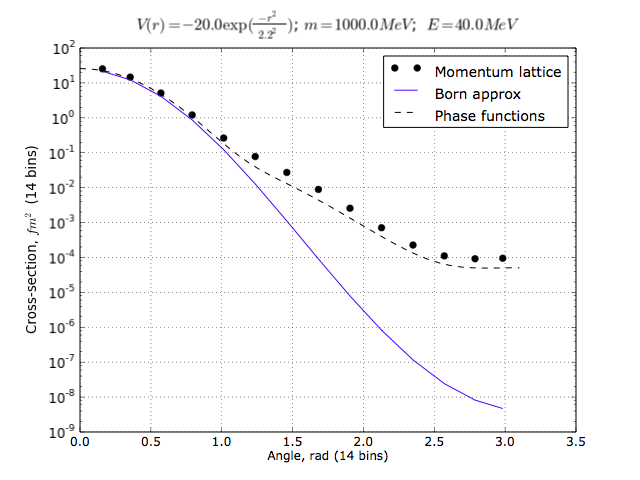
\includegraphics[width=0.75\linewidth]{gauss-high.png}}
  \caption{Сечение рассеяния на модельном гауссовом потенциале. $m$=1000MeV, $E$=40MeV, $V(r)=-20\exp(\frac{-r^2}{2.2^2}) [\text{MeV}]$. Решетка 14х14.}
  \label{fig:skatter11}
  \end{figure}
  
	\begin{figure}[h!]
  \center{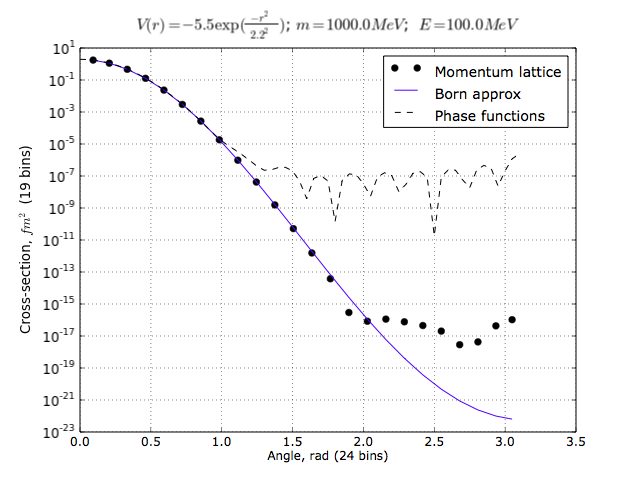
\includegraphics[width=0.75\linewidth]{gauss-low.png}}
  \caption{Сечение рассеяния на модельном гауссовом потенциале. $m$=1000MeV, $E$=100MeV, $V(r)=-5.5\exp(\frac{-r^2}{2.2^2}) [\text{MeV}]$. Решетка 19х24.}
  \label{fig:skatter12}
  \end{figure}
	
	В качестве сравнительного теста используем потенциал в виде гауссового пика.
	\begin{equation}
	   V(r) = A e^{-r^2/a^2},
	\end{equation}
	и соостветственно
	\begin{equation}
	   V(\vect{q'},\vect{q}) = \frac{Aa^3}{8\pi^{3/2}}\exp\big( - \frac{a^2}{4}(\vect{q'}-\vect{q})^2 \big)
	\end{equation}
	Интегрирование по $\varphi$ в соответствии с (\ref{phi_int}) может быть проведено аналитически
	\begin{equation}
	   W(\vect{q_2},\vect{q_1}) = \frac{Aa^3}{4\pi^{1/2}} e^{ - a^2( q_1^2 + q_2^2 - 2q_1q_2\cos\theta_1\cos\theta_2)/4 }
	    I_0 \big( a^2q_1q_2\sin\theta_1\sin\theta_2/2 \big)
	\end{equation}
	где $I_0$ -- модифицированная функция Бесселя.
	
	На рисунке \ref{fig:skatter11} сравниваются результаты расчетов сечений упругого рассеяния, найденных в нашем трёхмерном подходе (на импульсной решетке) с методом суммирования ряда по парциальным амплитудам и первым Борновским приближением. Хорошо видно что, результаты вычисления при малых энергиях совпадают с результатом метода фазовых функций. 
	
	На рисунке \ref{fig:skatter12} приведен результат аналогичного расчета в области применимости борновского приближения. Видно, что метод волновых пакетов обеспечивает большую точность чем метод фазовых функций. Это связано с тем, что в методе фазовых функций при вычислении сечения приходится суммировать сильно осциллирующие функции.


\subsection{Расчет для потенциала Мальфлие-Тьона.}
\begin{figure}[h!]
\center{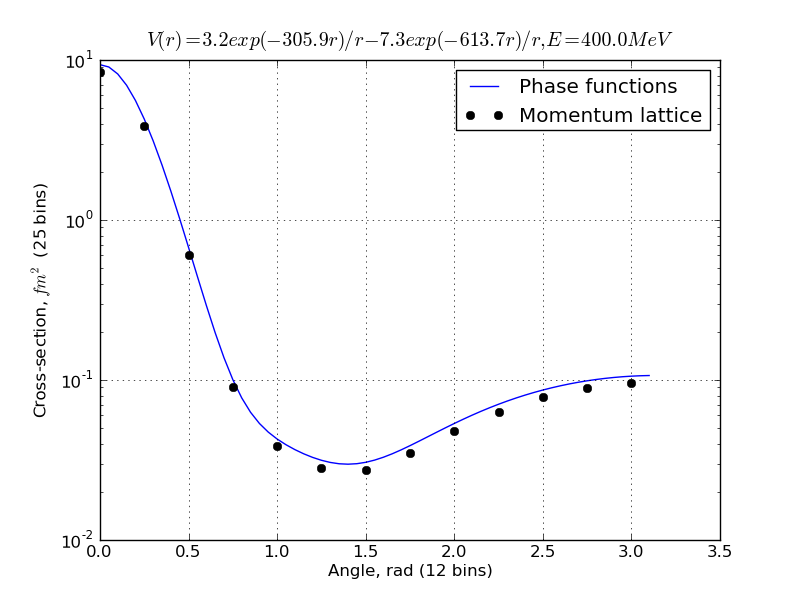
\includegraphics[width=0.8\linewidth]{malfliet-high.png}}
\caption{Сечение рассеяния на потенциале Мальфлие-Тьона. $m$=469MeV, $E$=400MeV, $V(r)=3.2\exp(-305.9r)/r-7.3\exp(-613.7r)/r [\text{MeV}]$. Решетка 25х12. }
\label{fig:skatter21}
\end{figure}

\begin{figure}[h!]
\center{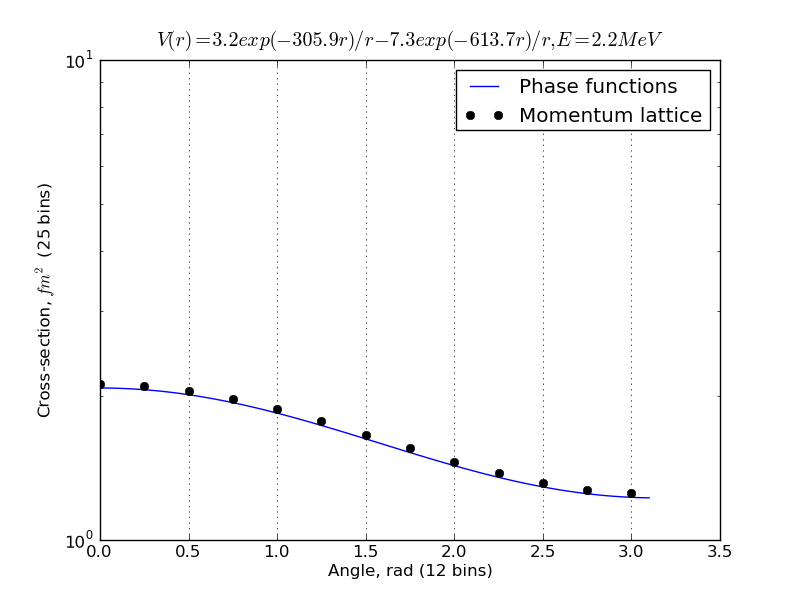
\includegraphics[width=0.8\linewidth]{malfliet-low.png}}
\caption{Сечение рассеяния на потенциале Мальфлие-Тьона. $m$=469MeV, $E$=2.2MeV, $V(r)=3.2\exp(-305.9r)/r-7.3\exp(-613.7r)/r [\text{MeV}]$. Решетка 25х12.}
\label{fig:skatter22}
\end{figure}


В качестве более реалистичного примера возьмем N-N потенциал Мальфлие-Тьона
\[
V(r) = V_R\frac{-\mu_Rr}{r} - V_A\frac{-\mu_Ar}{r}
\]
и соответственно в импульсном представлении
\[
V(\vect{q'},\vect{q}) = \frac{1}{2\pi^2}\bigg( \frac{V_R}{(\vect{q'}-\vect{q})^2+\mu_R^2} + \frac{V_A}{(\vect{q'}-\vect{q})^2+\mu_A^2} \bigg)
\]

Интегрирование по формуе \ref{phi_int} может быть выполнено аналитически
\begin{multline}
W(q',q,\theta',\theta) = \frac{1}{\pi}\bigg[ \frac{V_R}{\sqrt{(q'^2+q^2-2qq'cos(\theta')cos(\theta)+\mu_R)^2 - 4q'^2q^2sin^2(\theta')sin^2(\theta) }} \\ +  \frac{V_R}{\sqrt{(q'^2+q^2-2qq'cos(\theta')cos(\theta)+\mu_A)^2 - 4q'^2q^Asin^2(\theta')sin^2(\theta) }} \bigg]
\end{multline}
В данном случае результаты решения так же согласуются с методом фазовых функций (рисунки \ref{fig:skatter21} и \ref{fig:skatter22}).

\newline
\section{Заключение}

В данной работе развит формализм для описания рассеяния без разложения по парциальным волнам. В качестве базисных состояний используются волновые пакеты полученные интегрированием по малым клеткам в импульсном пространстве. Отдельно рассмотрен случай аксиально-симметричных волновых пакетов, так как они возникают при рассеянии на центральных потенциалах. Получены формулы для произвольных операторов в представлении волновых пакетов, для функции Грина. Записано уравнение Липпманна-Швингера в представлении волновых пакетов.

Вычислено сечение рассеяния на двух потенциалах при различных энергиях. Результаты согласуются с методом фазовых функций, что позволяет утверждать о правильных результатах расчета по данному методу.


\pagebreak
\addcontentsline{toc}{section}{Список литературы.} 
\begin{thebibliography}{9}

\bibitem{elster}
  Ch. Elster, J.H..Thomas, W. Gloeckle,
  \emph{Two-Body T-Matrices without Angular Momentum Decomposition: Energy and Momentum Dependencies}.
  Few Body Syst. 24 (1998) 55-79

\bibitem{kuku1}
  O. A. Rubtsova, V. N. Pomerantsev, and V. I. Kukulin,
  \emph{Quantum scattering theory on the momentum lattice}.
  10.1103/PhysRevC.79.064602

\bibitem{kuku2}
  В. И. Кукулин, О. А. Рубцова,
  \emph{Дискретная квантовая теория рассеяния}.
  ТМФ, 134:3 (2003), 460–486 

\bibitem{sakurai}
  J.J. Sakurai,
  \emph{Modern Quantum Mechanics}.
  Addison Wesley, Massachusetts,
  2nd Edition,
  1994.

\bibitem{babik}
  В.В. Бабиков,
  \emph{Метод фазовых функций в квантовой механике}.
  УФН, 1967, 5/a

\end{thebibliography}


    
\end{document}

